\chapter{Organisation}

Dieses Kapitel beschreibt kurz die Stakeholder des Projekts sowie den allgemeinen Aufbau.

\section{Projektbeteiligte}

\begin{table}[H]
	\centering
	\begin{tabular}{p{0.3\textwidth} p{0.2\textwidth} p{0.3\textwidth}}
	\textbf{Name} & \textbf{Funktion} & \textbf{E-Mail Adresse} \\ \midrule
	Simon Meer & Student & simon.meer@students.bfh.ch \\
	Prof. Urs K�nzler & Betreuer & urs.kuenzler@bfh.ch \\
	Yves Petitpierre & Experte & yves.petitpierre@ericsson.com \\
	\end{tabular}
\end{table}

\section{Projektmanagement}

\begin{itemize}
	\item Das Projekt wird innerhalb eines \gls{git}-Projektes gef�hrt. Ein privater, zentraler Klon wird auf GitHub abgelegt, welches unter der Adresse \url{https://github.com/EusthEnoptEron/IMVR} erreichbar ist.
	\item Meetings zwischen dem Studenten und dem Betreuer finden jeden zweiten Mittwoch in Biel statt.
	\item Gearbeitet wird durch den Studenten Montags bis Donnerstags an einem Arbeitsplatz im CPVR Labor in Biel.
	\item Das Projekt wird in Scrum-�hnlich mit Sprints vorangetrieben.
\end{itemize}

\begin{landscape}
	\section{Ordnerstruktur}
	
	\begin{figure}[H]
		\centering
		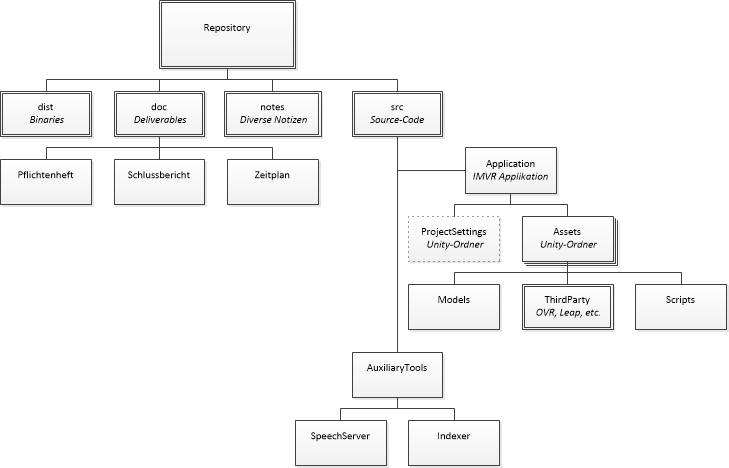
\includegraphics{bilder/file_structure}
		\caption{Die Ordnerstruktur des Projektes.}	
	\end{figure}
\end{landscape}

\begin{landscape}
	\section{Zeitplan}
	\begin{figure}[H]
		\centering
		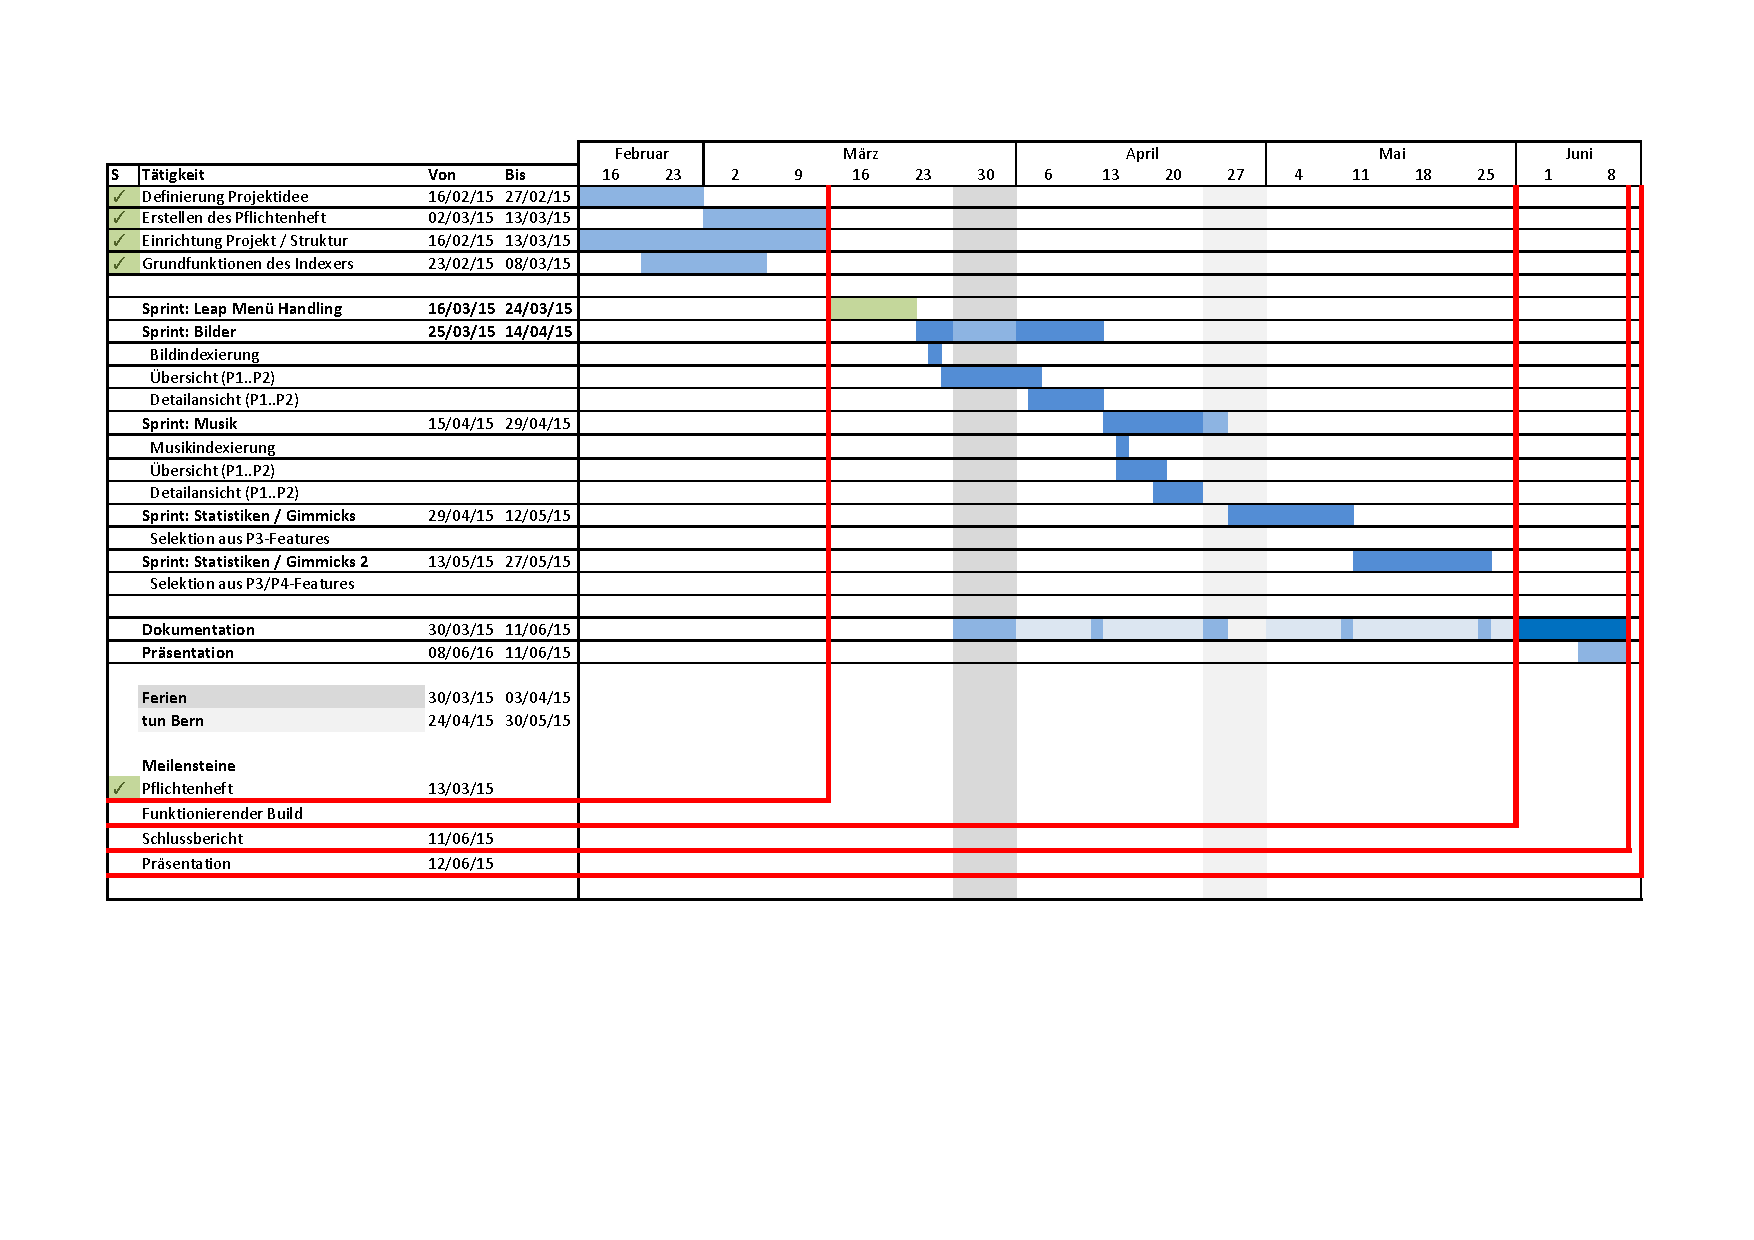
\includegraphics[trim=10mm 55mm 10mm 20mm, clip=true, width=1.1\linewidth]{../Zeitplan/Zeitplan}
		\caption{Der Zeitplan mit Sprints und Priorit�ten.}
	\end{figure}
	
\end{landscape}

